\section{Supplementary results}
\label{app:tables}

Table~\ref{tab:scores}: every instrument at every iteration under the training oracle (the held-out
judge's version is Table~\ref{tab:scores-heldout} in Appendix~\ref{app:heldout}, which collects
that judge's results). Figure~\ref{fig:overpraise}: the keyword marker of \S\ref{sec:therapist}.
Figure~\ref{fig:responsiveness}: the therapist's four replies of Table~\ref{tab:process} by
iteration under both judges. Figure~\ref{fig:textspace}: the two runs in sentence-embedding space
(Figure~\ref{fig:textspace-body} and a third measure). Figure~\ref{fig:forest}: the session-level
behaviour-channel profile. Figure~\ref{fig:tails}: the $\Kf$ rollout audit, summarised in the
Limitations. Over the $121{,}088$ logged $\Kf$ candidates ($88\%$ of those scored), $82\%$ of
rollouts ran the full five turns; the early-ending share ranged from $12\%$ at iteration 10 to
$30\%$ at iteration 6, and in $16\%$ of candidates the patient closed the session. Early-ending
candidates scored at or below their group mean (by up to $0.09$ points, depending on how the
rollout ended) and were the group's best less often than chance ($0.10$ vs.\ $0.125$).

\begin{table*}[t]
\centering
\footnotesize
\setlength{\tabcolsep}{4.5pt}
\renewcommand{\arraystretch}{0.92}
\begin{tabular}{@{}lrrrrrrrrr@{}}
\toprule
Iteration & \QQ & Q1 & Q2 & WAI-SR & CSQ-8 & MI-SAT & MITI & PCT & MICI ($\downarrow$)\\
\midrule
Base & $3.015$ & $2.966$ & $3.064$ & $2.873$ & $2.359$ & $2.837$ & $3.172$ & $0.479$ & $0.210$\\
\midrule
\multicolumn{10}{@{}l}{\emph{$K{=}0$}}\\
1 & $3.269$ & $3.177$ & $3.361$ & $2.976$ & $2.477$ & $2.986$ & $3.284$ & $0.481$ & $0.228$\\
2 & $3.359$ & $3.302$ & $3.417$ & $3.004$ & $2.514$ & $3.054$ & $3.495$ & $0.503$ & $0.169$\\
3 & $3.993$ & $3.935$ & $4.051$ & $3.301$ & $2.811$ & $3.425$ & $3.938$ & $0.544$ & $0.230$\rlap{$^{*}$}\\
4 & $4.004$ & $3.898$ & $4.111$ & $3.292$ & $2.751$ & $3.410$ & $4.039$ & $0.552$ & $0.251$\\
5 & $3.972$ & $3.869$ & $4.075$ & $3.208$ & $2.715$ & $3.321$ & $3.940$ & $0.522$ & $0.277$\\
6 & $3.966$ & $3.810$ & $4.121$ & $3.297$ & $2.710$ & $3.306$ & $4.010$ & $0.530$ & $0.255$\\
7 & $4.074$ & $3.946$ & $4.202$ & $3.318$ & $2.757$ & $3.418$ & $4.102$ & $0.551$ & $0.270$\\
8 & $4.082$ & $3.935$ & $4.229$ & $3.374$ & $2.749$ & $3.441$ & $4.234$ & $0.572$ & $0.535$\\
9 & $3.807$ & $3.529$ & $4.086$ & $3.089$ & $2.486$ & $3.050$ & $3.938$ & $0.450$ & $0.350$\\
10 & $3.753$ & $3.606$ & $3.899$ & $3.438$ & $2.773$ & $3.479$ & $3.922$ & $0.574$ & $0.838$\\
\midrule
\multicolumn{10}{@{}l}{\emph{$K{=}5$}}\\
1 & $3.272$ & $3.173$ & $3.370$ & $2.964$ & $2.396$ & $2.946$ & $3.299$ & $0.477$ & $0.228$\\
2 & $3.435$ & $3.360$ & $3.510$ & $3.044$ & $2.582$ & $3.144$ & $3.536$ & $0.515$ & $0.228$\\
3 & $3.862$ & $3.806$ & $3.917$ & $3.320$ & $2.831$ & $3.490$ & $3.865$ & $0.580$ & $0.308$\\
4 & $4.120$\rlap{$^{*}$} & $4.100$\rlap{$^{*}$} & $4.140$ & $3.441$ & $2.921$\rlap{$^{*}$} & $3.622$\rlap{$^{*}$} & $4.083$ & $0.614$\rlap{$^{*}$} & $0.305$\\
5 & $4.042$ & $3.988$ & $4.096$ & $3.464$\rlap{$^{*}$} & $2.908$\rlap{$^{*}$} & $3.559$\rlap{$^{*}$} & $4.010$ & $0.578$\rlap{$^{*}$} & $0.340$\\
6 & $4.229$\rlap{$^{*}$} & $4.200$\rlap{$^{*}$} & $4.258$ & $3.543$\rlap{$^{*}$} & $2.935$\rlap{$^{*}$} & $3.682$\rlap{$^{*}$} & $4.250$\rlap{$^{*}$} & $0.625$\rlap{$^{*}$} & $0.281$\\
7 & $4.270$\rlap{$^{*}$} & $4.206$\rlap{$^{*}$} & $4.334$ & $3.529$\rlap{$^{*}$} & $2.977$\rlap{$^{*}$} & $3.663$\rlap{$^{*}$} & $4.284$\rlap{$^{*}$} & $0.621$\rlap{$^{*}$} & $0.248$\\
8 & $4.254$\rlap{$^{*}$} & $4.200$\rlap{$^{*}$} & $4.309$ & $3.579$\rlap{$^{*}$} & $2.924$\rlap{$^{*}$} & $3.639$\rlap{$^{*}$} & $4.312$ & $0.627$\rlap{$^{*}$} & $0.197$\rlap{$^{*}$}\\
9 & $4.454$\rlap{$^{*}$} & $4.408$\rlap{$^{*}$} & $4.501$\rlap{$^{*}$} & $3.661$\rlap{$^{*}$} & $3.078$\rlap{$^{*}$} & $3.847$\rlap{$^{*}$} & $4.521$\rlap{$^{*}$} & $0.699$\rlap{$^{*}$} & $0.212$\rlap{$^{*}$}\\
10 & $4.517$\rlap{$^{*}$} & $4.465$\rlap{$^{*}$} & $4.570$\rlap{$^{*}$} & $3.729$\rlap{$^{*}$} & $3.062$\rlap{$^{*}$} & $3.832$\rlap{$^{*}$} & $4.536$\rlap{$^{*}$} & $0.685$\rlap{$^{*}$} & $0.210$\rlap{$^{*}$}\\
\bottomrule
\end{tabular}
\caption{\textbf{Every instrument at every iteration} under the training oracle: the mean over the
96 personas (the Base: over its 192 conversations, two per persona). A star marks the better run at
an iteration where the persona-paired $\Kf$ vs.\ $\Kz$ contrast on that instrument is significant
(Holm across iterations 1--10 within instrument); the only star on a $\Kz$ cell is MICI at
iteration 3. MICI is lower-is-better. The iteration-10 rows are Table~\ref{tab:endpoint};
Figure~\ref{fig:headline} draws the columns.}
\label{tab:scores}
\end{table*}

\begin{figure}[!htb]
\centering

\includegraphics[width=0.47\textwidth]{figures/overpraise_judgefree_grpo.png}
\caption{The keyword marker of \S\ref{sec:therapist} by iteration: the share of therapist turns
containing at least one of ten praise phrases (Appendix~\ref{app:marker}), no model in the loop.
Iteration 0 is the Base.}
\label{fig:overpraise}
\end{figure}

\begin{figure*}[t]
\centering
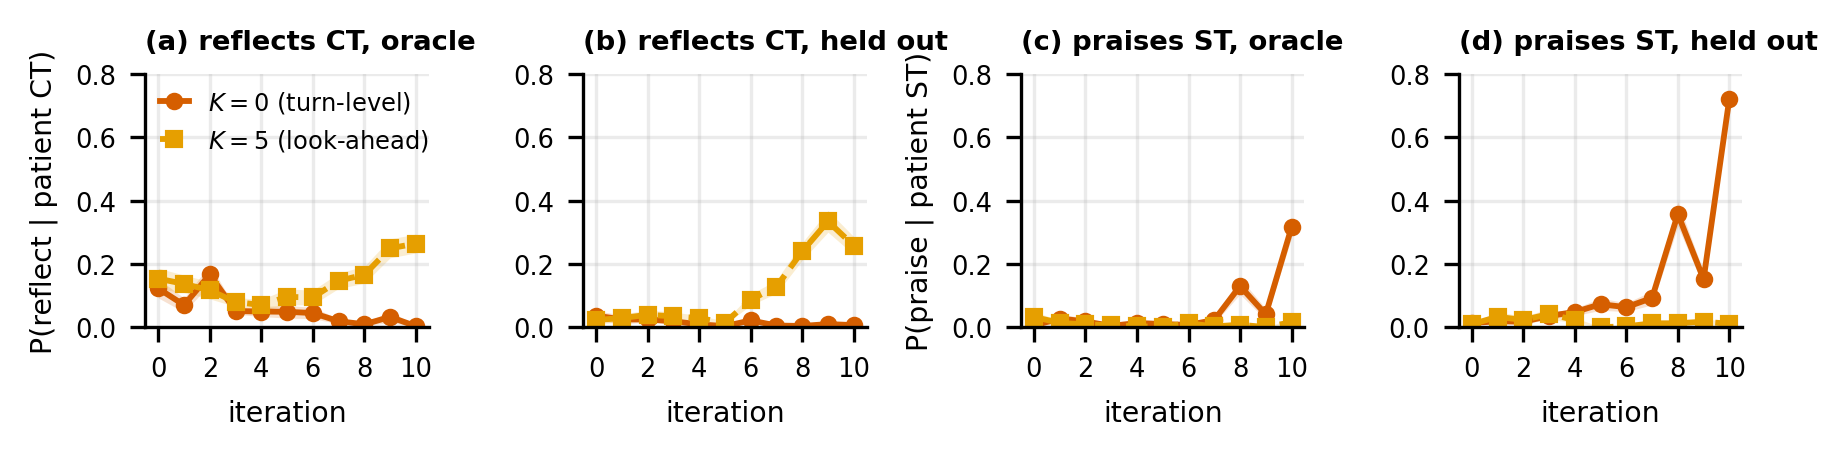
\includegraphics[width=0.94\textwidth]{figures/responsiveness_grpo.png}
\caption{The therapist's replies by iteration, under the training oracle (top) and the held-out
judge (bottom): mean $\pm$ SE over the conversations in which the patient's utterance occurred.
\textbf{(a, e)} The share of the patient's change-talk (CT) utterances the therapist answers with a
reflection. \textbf{(b, f)} The share of the patient's sustain-talk (ST) utterances it answers
with non-specific praise, \textbf{(c, g)} with persuasion, and \textbf{(d, h)} with a reflection.
The iteration-10 values are the middle blocks of Tables~\ref{tab:process}
and~\ref{tab:process-heldout}.}
\label{fig:responsiveness}
\end{figure*}

\begin{figure*}[t]
\centering
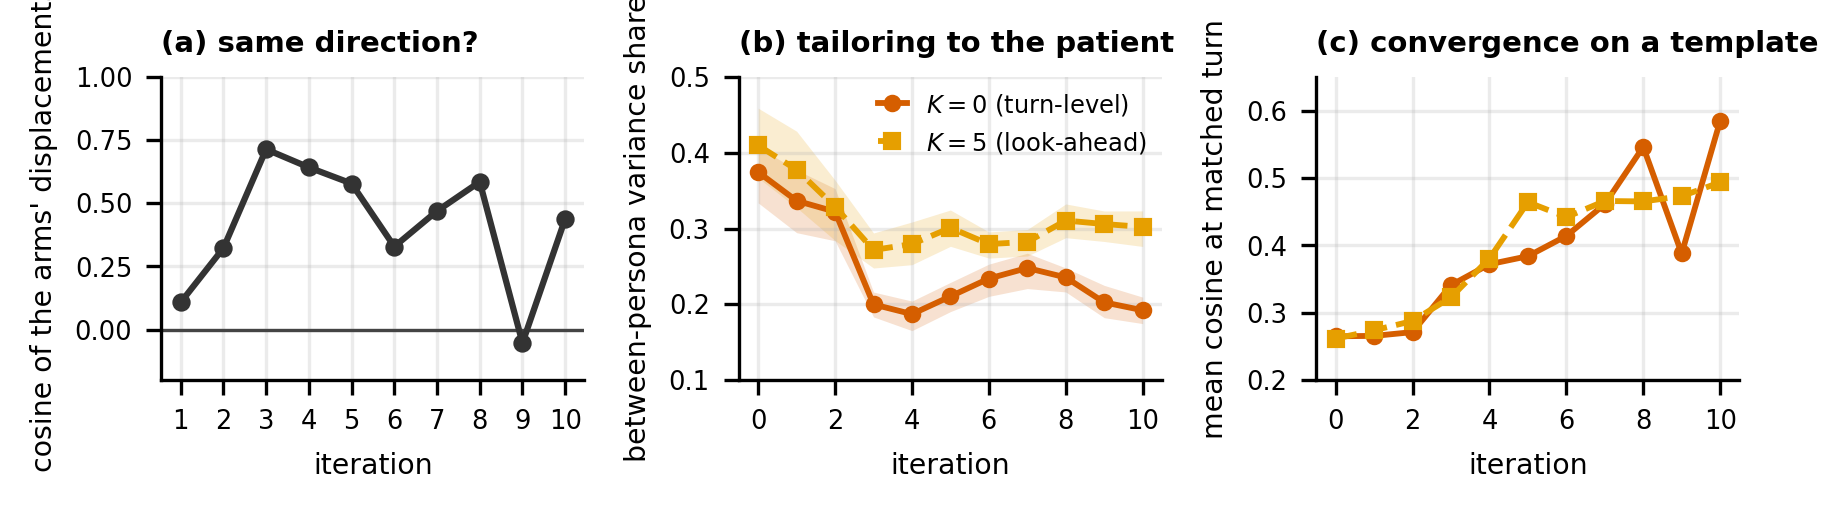
\includegraphics[width=0.94\textwidth]{figures/text_grpo.png}
\caption{The two runs in sentence-embedding space (every therapist turn embedded with
\texttt{all-MiniLM-L6-v2}; the scripted opener excluded); panels (a) and (b) are
Figure~\ref{fig:textspace-body}. \textbf{(a)} The cosine between the two runs' moves away from
the Base's mean embedding at each iteration: $1$ would mean they learned the same thing.
\textbf{(b)} The share of embedding variance that lies between conversations, a measure of how
much the therapist's turns depend on which patient it is talking to, with a $95\%$ bootstrap band
over conversations. \textbf{(c)} The mean pairwise cosine between turns at the same position in
different conversations: convergence on a template.}
\label{fig:textspace}
\end{figure*}

\begin{figure*}[p]
\centering

\includegraphics[width=0.92\textwidth]{figures/k_channel_forest_grpo_gpt-4o-mini.png}
\caption{Every behaviour channel at iteration 10 under the training oracle's session-level coders:
the persona-paired contrast $\Kf - \Kz$ as \dz\ ($n{=}96$; positive means the $\Kf$ policy does
more of it; hollow bars are not significant). Over-praise is the dominant channel by a wide
margin, followed by affirmations; the channels the $\Kf$ policy does more of are questions and,
among the MI-inconsistent codes, direct/order and persuasion. The share of MI-consistent codes is
\emph{lower} under $\Kf$ because the MITI coder counts every affirmation as MI-adherent, earned or
not. Every channel is shown so that substitution, MI-inconsistency moving to another channel
rather than falling, would be visible rather than hidden by the total.}
\label{fig:forest}
\end{figure*}

\begin{figure*}[t]
\centering

\includegraphics[width=0.96\textwidth]{figures/tail_audit_grpo.png}
\caption{The $\Kf$ rollout audit, over the $121{,}088$ logged candidates ($88\%$ of those
scored). A rollout is meant to add five turns after the candidate; it is cut short when the
patient closes the session or when the policy's own turn inside the rollout ends it.
\textbf{(a)} How often that happened, by training iteration ($95\%$ bootstrap intervals; pooled
$18\%$), and how much of it was the patient closing the session ($16\%$). \textbf{(b)} What a
cut-short rollout cost the candidate: its reward minus the mean of its group, by how many turns
were actually simulated and who ended them (\emph{pat.}: the patient closed the session;
\emph{pol.}: the policy's own turn ended it; \emph{none}: the candidate itself ended the session).
Candidates whose rollout ran all five turns sit at the group mean, those the patient closed sit
close to it, and those the policy's own turn ended sit about $0.09$ below. \textbf{(c)} How often
a candidate was its group's best, separately for rollouts that ran to length and rollouts that
were cut short; the dotted line is chance, $1/8$. Read together: the lever was applied as
specified in most cases, and a rollout that ended early cost the candidate a little, which is the
keep-the-session-open pressure discussed in the Limitations.}
\label{fig:tails}
\end{figure*}
